\let\negmedspace\undefined
\let\negthickspace\undefined
\documentclass[journal]{IEEEtran}
\usepackage[a5paper, margin=10mm, onecolumn]{geometry}
\setlength{\headheight}{1cm} % Set the height of the header box
\setlength{\headsep}{0mm}     % Set the distance between the header box and the top of the text

\usepackage{gvv-book}
\usepackage{gvv}
\usepackage{cite}
\usepackage{amsmath,amssymb,amsfonts,amsthm}
\usepackage{algorithmic}
\usepackage{graphicx}
\usepackage{textcomp}
\usepackage{xcolor}
\usepackage{txfonts}
\usepackage{listings}
\usepackage{enumitem}
\usepackage{mathtools}
\usepackage{gensymb}
\usepackage{comment}
\usepackage[breaklinks=true]{hyperref}
\usepackage{tkz-euclide} 
\usepackage{listings}
\usepackage[latin1]{inputenc}                                
\usepackage{color}                                            
\usepackage{array}                                            
\usepackage{longtable}                                       
\usepackage{calc}                                             
\usepackage{multirow}                                          
\usepackage{hhline}                                           
\usepackage{ifthen}                                           
\usepackage{lscape}
\usepackage{float}

\begin{document}
	\bibliographystyle{IEEEtran}
	\vspace{3cm}
	\title{11.16.4.3.3}
	\author{EE24BTECH11022 - Eshan Sharma}
	{\let\newpage\relax\maketitle}
	\renewcommand{\thefigure}{\theenumi}
	\renewcommand{\thetable}{\theenumi}
	\setlength{\intextsep}{10pt} % Space between text and floats
	
	\textbf{Question:}  
	A die has two faces each with number '1', three faces each with number '2', and one face with number '3'. If the die is rolled once, determine \( P(\text{not } 3) \).  
	
	\textbf{Theoretical Solution:}  
	The die has 6 faces in total. The probability of rolling a number other than `3` is:
	\[
	P(\text{not } 3) = 1 - P(3)
	\]
	From the problem, the probability of rolling `3` is:
	\[
	P(3) = \frac{\text{Number of faces with 3}}{\text{Total faces}} = \frac{1}{6}
	\]
	Thus:
	\[
	P(\text{not } 3) = 1 - \frac{1}{6} = \frac{5}{6} \approx 0.8333
	\]
	
	\textbf{Numerical Solution using Monte Carlo Method:}  
	The Monte Carlo method is used to estimate \( P(\text{not } 3) \). This involves simulating a large number of die rolls and counting the proportion of rolls that result in a number other than `3`.
	
	\textbf{Steps of the Simulation:}  
	\begin{enumerate}
		\item Generate a large number \( N \) of random numbers uniformly distributed between 0 and 1.
		\item Map these numbers to die outcomes based on the given probabilities:
		\begin{align*}
			\text{Face `1`: } & \text{Range } [0, 2/6) \\
			\text{Face `2`: } & \text{Range } [2/6, 5/6) \\
			\text{Face `3`: } & \text{Range } [5/6, 1)
		\end{align*}
		\item Count the number of outcomes where the result is not `3`.
		\item Estimate \( P(\text{not } 3) \) as the ratio of outcomes not equal to 3 to the total number of rolls:
		\[
		P(\text{not } 3) \approx \frac{\text{Count of outcomes not equal to 3}}{N}
		\]
	\end{enumerate}
	
	\textbf{Plots:}  
	\begin{figure}[H]
		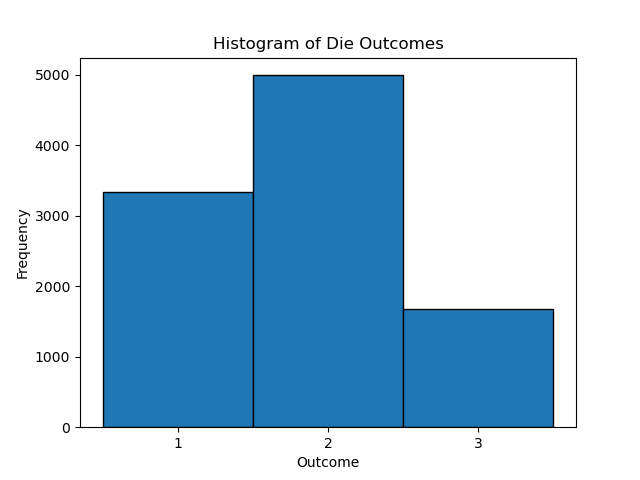
\includegraphics[width=\columnwidth]{figs/fig.png}
		\caption{Stem Plot of Monte Carlo Simulation for \( P(\text{not } 3) \).}
	\end{figure}
	
	\begin{figure}[H]
		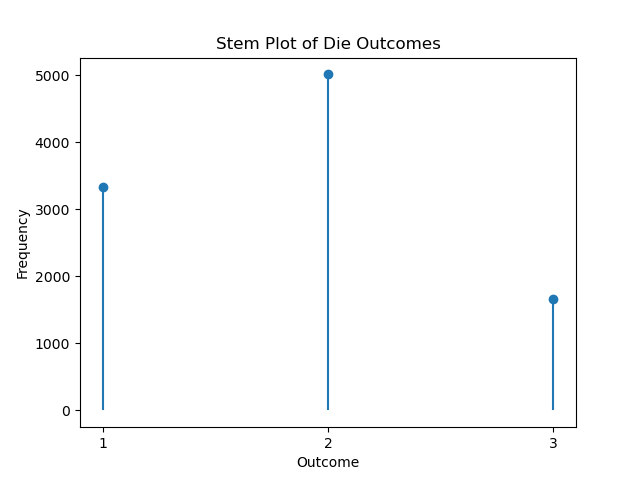
\includegraphics[width=\columnwidth]{figs/fig2.png}
		\caption{Histogram of Simulated Outcomes.}
	\end{figure}
	
	\textbf{Explanation of Plots:}  \\
	\textbf{1. Stem Plot of Monte Carlo Simulation:}  
	- \textbf{Purpose:} This plot shows the estimated probability of \( P(\text{not } 3) \) over multiple iterations of the simulation.
	- \textbf{X-axis:} Iteration number (or step number) in the simulation.  
	- \textbf{Y-axis:} Cumulative estimate of \( P(\text{not } 3) \) after each iteration.  
	- \textbf{Key Insight:}  
	- The values fluctuate initially due to randomness.  
	- As the number of iterations increases, the estimate converges to the theoretical value \( \frac{5}{6} \).  
	- \textbf{Usage:} This helps visualize the stability and convergence of the simulation.  
	
	\textbf{2. Histogram of Simulated Outcomes:}  
	- \textbf{Purpose:} Visualizes the frequencies of outcomes from the simulated rolls.  
	- \textbf{X-axis:} Possible outcomes (1, 2, or 3).  
	- \textbf{Y-axis:} Frequency of each outcome.  
	- \textbf{Key Insight:}  
	- The frequency of outcomes `1` and `2` combined is higher than `3`, aligning with \( P(\text{not } 3) = \frac{5}{6} \). \\ 
	- \textbf{Usage:} Validates that the simulation adheres to the die's probabilities.  
	
\end{document}
